\subsection{Practical algorithm}
\label{ssec:practical}

We start by defining a similar structure as the augmented graph, but more amenable to practical purposes.
The graph $G^B$ defined in section \ref{sec:augmented} may contain a lot of redundant information, hence it is not a minimal representation.
For example, the same efficient path $uv$ can be repeated many times in the form $\pp{u,1}\pp{v,0}$, $\pp{u,2}\pp{v,1}$ and so on.
By encoding this information more efficiently, we can reduce the size of the augmented graph and obtain considerable improvements both in query time and in data storage.

We construct an augmented graph without this duplicated information as follows.
The nodes are, as before, pairs $\pp{v,b}$, but an edge $\pp{v,b},\pp{v',b'}$ is placed only if it is essential for some efficient path, i.e., removing said edge changes the correctness of a query.
If we let $\Pst^E$ be the set of all efficient paths from $s$ to $t$, we take every $P\in \Pst^E$ with cost $b\leq B$ and trace it in the augmented graph.
The tracing is such that the augmented path is forced to end at $\pp{t,0}$.
In other words, all efficient paths $P\in \Pst^E$ can be represented by a set a set of efficient paths ending at $\pp{t,0}$. 

\begin{definition}\label{def:pruned_aug_graph}
The pruned augmented graph is defined by $\Gp^B=(\Vp^B,\Ep^B)$, where
\begin{align*}
\Vp^B &:=\{\pp{v,b}: v\in V, b=0,1,\ldots,B\},\\
\Ep^B &:=\{\pp{v,b}\pp{v',b'} : \exists s,t\in V, P\in\PE_{s,t}, c(P)\leq B, \\
&\qquad vv'\in P, b=c(P[v,t]), b'=c(P[v',t])  \}.
\end{align*}
In $\Gp^B$ all the lengths are preserved.
\end{definition}
Note that in $\Gp^B$ there are no sink nodes, hence it has at least $n$ nodes and $nB$ arcs fewer compared to $G^B$.
In the worst case, those $nB$ arcs are the only gain by doing this process.
Nevertheless, in practice this graph can be up to 40\% smaller than $G^B$.
Observe that, by running Dijkstra in $G^B$, $\Gp^B$ can be computed in time $\Or(n^2B\log(nB))$.

\subsubsection{HD of the pruned augmented graph}

A shortest path in $\Gp$ does not necessarily project to an efficient path, even if the path ends in a node of the form $\pp{t,0}$.
In contrast, if $P$ projects to an efficient path, then necessarily $P$ is shortest. 
To bound the HD, the correct system to study is
\[
\tilde\PB:=\{P: P\text{ ends in a node }\pp{t,0}, \bar P\in \PE, c(\bar P)\leq B \}.
\]
The following result shows how the HD of this system relates to that of $\PE$.
We omit the proof since it is identical as the one in Proposition~\ref{prop:HDaugmented}.
\begin{proposition}
The HD of $\tilde\PB$ is $Bh_c$, where $h_c$ is the HD of $\PE$.
\end{proposition}

\subsubsection{Description of the practical algorithm}

We use techniques described in \cite{hubimplem} combined with an approach tailored for augmented graphs.
The main idea is to first use contraction hierarchies to get a node ranking and then define the forward hubs of a node as the nodes visited during a contraction-based forward search.
The reverse hub is defined analogously.
These are valid hubs, since the highest rank node in a path is guaranteed to be in both hubs.

The most important parameter in CH is the rank; results vary greatly from one choice of ranks to another.
We obtain a rank in $G$ by running a greedy shortest-path cover, defined as follows.
Start with a cover $C=\varnothing$ and compute the set of all shortest paths $\PS$.
Take a node $v\notin C$ hitting most paths in $\PS$, then remove all those paths from $\PS$, add $v$ to $C$ and iterate.
The rank is defined as $n$ for the first node added to $C$, $n-1$ for the second and so on.

We work with the pruned augmented graph $\tilde G_B$, which takes some time to compute, but yields considerably better hubs. 
Recall that in $\tilde G_B$ there are no sink-nodes nor ``replicated information'', since efficient paths are stored just once.
Given a rank for nodes in $G$, we contract $\tilde G_B$ as follows.
Say that $V$ is ordered according to the rank, so node $1$ is the least important and $n$ the most important.
In $\tilde G_B$, we first contract the nodes $\pp{1,b}$ for $b=B,\ldots,0$, then the nodes $\pp{2,b}$ and so on till the nodes $\pp{n,b}$ are the last to contract. 

To obtain better hubs we prune the results obtained by contraction-based searches.
If $w$ is in the forward search of $v$ with distance $d$, it might be that $\dist(v,w)<d$, this occurs because the search goes only to higher rank nodes and the discovered path is missing some node.
When $\dist(v,w)<d$, we can safely remove $w$ from the hub of $v$, since the highest ranked node in a shortest path will have the correct distance.
The entire process can be summarized in the following steps.

\begin{enumerate}[nosep]
\item Compute the shortest paths in $G$ and use a greedy approach to obtain a cover $C$
\item Compute the pruned augmented graph $\tilde G_B$
\item Contract $\tilde G_B$ using the rank induced by $C$
\item Create hubs $\Lf(v),\Lb(v)$ using CH
\item Prune the hubs by running HL queries between $v$ and nodes in $\Lf(v)$. 
Run a similar process for $\Lb(v)$.
\end{enumerate}
Note that in the last step we bootstrap HL to improve it.
This works because the fact that some nodes have incorrect distance labels does not impact the correctness of a HL query; a node minimizing the distance is returned and such node must have a correct label.

\begin{remark}
For the first step, a direct approach requires to store in memory all the shortest paths.
In many cases, this can impose a prohibitive memory requirement.
There are two ways around this issue.
We can compute the cover by processing one shortest path tree at a time, this translates to $\Omega(n^3\log n)$ running time, but $\Or(n)$ memory.
The second approach we suggest is to compute only $k<<n$ shortest path trees and cover these greedily.
We use an off-the-shelf clustering method to obtain $k$ cluster centers, from which we compute the shortest paths. 
As shown in Figure~\ref{fig:clusters}, the clustering approach provide a very good approximation of the hubs with even a relatively small $k$.
\end{remark}

\begin{figure}
\begin{tikzpicture}[trim axis left]
\begin{axis}[
	scale only axis,
	height=3cm,
	width=3.9cm,
	xtick distance=300,
	ytick distance=1,	
	xmin = 10, xmax =1000,
	xlabel={Number of clusters},
	ylabel={},
	every axis plot/.append style={thick}]
\addplot[mark size=0.3,draw=black, mark=square*] table {tab_avg_sf.dat};
\addplot[mark size=0.3,draw=red, mark=triangle*] table {tab_max_sf.dat};
\addplot[mark size=0.3,draw=blue, mark=diamond*] table {tab_shorts_sf.dat};

\legend{Avg hub size, Max hub size,\# shortcuts}
\end{axis}
\end{tikzpicture}

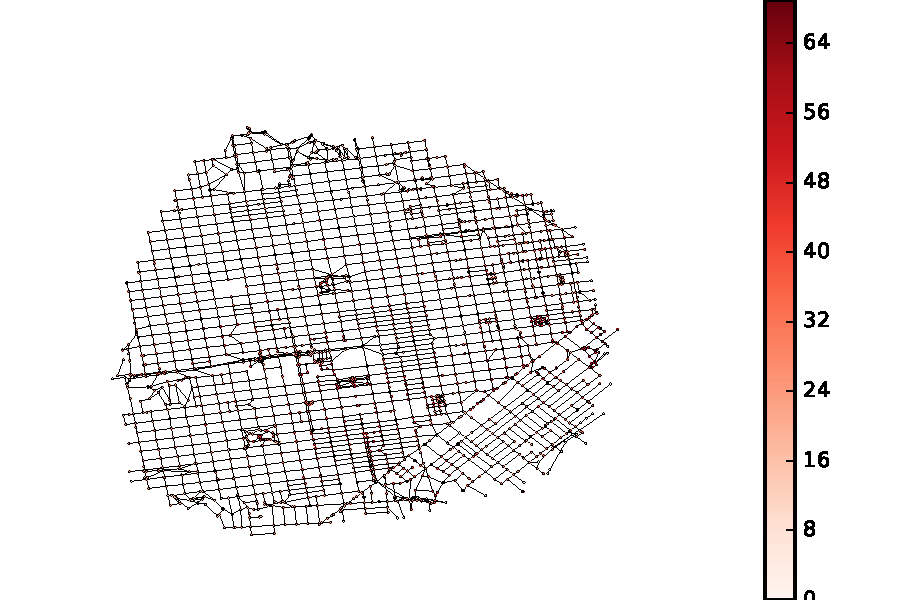
\includegraphics[clip, trim=14cm 3cm 3cm 3cm,scale=0.1]{TexImg/SF_hub_sizes.pdf}
\begin{tikzpicture}[trim axis left]
\begin{axis}[
	scale only axis,
	height=3cm,
	width=3.9cm,
	xtick distance=300,
	ytick distance=1,	
	xmin = 10, xmax =1000,
	xlabel={Number of clusters},
	ylabel={},
	every axis plot/.append style={thick}]
\addplot[mark size=0.3,draw=black, mark=square*] table {tab_avg_lu.dat};
\addplot[mark size=0.3,draw=red, mark=triangle*] table {tab_max_lu.dat};
\addplot[mark size=0.3,draw=blue, mark=diamond*] table {tab_shorts_lu.dat};

\legend{Avg hub size, Max hub size,\# shortcuts}
\end{axis}
\end{tikzpicture}

\caption{Performance of clustering for San Francisco (left) and Luxembourg (right). In the $y$-axis the quantities are normalized by the best greedy cover, i.e., using $k=n$.}
\label{fig:clusters}
\end{figure}

\subsubsection{Frontier and specific queries}

We test our algorithms with two different tasks.
Recall that the preprocess is done for some fixed value $B$ of maximum budget.
The first task is called a frontier query, for which, given $s$ and $t$, we must return the lengths of all efficient paths with costs $b=0,1,\ldots,B$.
The second is called a specific query, for given $s,t,b$ we return $\dist(s,t|b)$, i.e., only one efficient path.

Note that the pruned augmented graph $\Gp^B$ is designed for frontier queries.
To see this, fix the terminal $\pp{t,0}$.
As we ask for the shortest path from $\pp{s,B},\pp{s,B-1},\ldots,\pp{s,0}$ we are guaranteed to recover the entire frontier.
On the other hand, it may be that the shortest path between $\pp{s,b}$ and $\pp{t,0}$ does not correspond to $\dist(s,t|b)$.
This occurs when $b$ is not a tight budget and the efficient path requires less.

To answer specific queries, we modify $\Gp^B$ by adding extra edges.
For every $v\in V(G)$ and $b=1,2,\ldots,B$, we include the edge $\pp{v,b}\pp{v,b-1}$ with length $0$.
A simple argument shows that with the added edges, the shortest path between $\pp{s,b}$ and $\pp{t,0}$ has length $\dist(s,t|b)$

\subsection{Experiments} \label{sec:exp}
\todo{mention code is in github}
All the experiments were performed on a 64-bit desktop computer with a 3.40GHz Intel Core i7-6700 processor and 16GB RAM running Ubuntu 16.04.
The entire code is written in Python 2.7. We use the library Networkx for the graph representation and Dijkstra's algorithm.
To compute the SP cover we follow the exhibition in \cite{hubimplem}.

We evaluated the performance of our algorithms with real-world test networks: a small San Francisco network with 2643 nodes and 6588 edges for which real-world travel-time data was available as a Gaussian mixture model \cite{sf_data}, and a second (slightly larger) Luxembourg City network with 4026 nodes and 9282 edges for which travel-time distributions were synthesized from road speed limits \cite{niknami2016tractable}, as real-world data was unavailable.
 
In our experiments, we use the mean travel times for our length function and the following cost structure. The 10\% edges with the highest variance are assigned cost 1 and the rest cost 0.
This is a measure of risk, since edges with high variance are prone to cause a delay in the travel time.

\subsubsection{Runtime performance}


Tables~\ref{tab:sf_results} and \ref{tab:lu4k_results} present the CSP computation times for different maximum budgets $B$. 
For frontier queries, labelled as `f', the query times are measured as the average of 1000 random $s,t$.
For specific queries, labelled as `s', the times are measured as 1000 random triplets $s,t,b$.
The column for $B=0$ represents the original graph (without augmentation). 
As can be seen in the experimental results, our method finds the constrained shortest path solution on average four orders of magnitude faster than running Dijkstra's algorithm on the augmented graph. 
Preprocessing for frontier queries results in a more compact set of hub labels, since a node $\pp{s,b}$ needs to store information for paths with budget exactly equal to $b$.
On the other hand, for specific queries, $\pp{s,b}$ needs to store information for all budgets up to $b$.

The longer preprocessing time for frontier queries can be explained as follows.
There are many cases when two nodes are not reachable, to detect this requires Dijkstra to explore the entire graph.
In contrast, for specific queries we add extra edges $\pp{s,b}\pp{s,b-1}$, hence a reachability test ends, in average, earlier.
In the contraction step, we want to remove a node without altering the shortest path, a process that requires many reachability tests.

\begin{table*}
\begin{subtable}{.5\textwidth}
\begin{center}
\begin{tabular}{ | l | p{1cm} | p{1cm} | p{1cm} | p{1.2cm} | p{1.2cm} | }
\hline
	B & Preproc [m] & Avg F Size & Avg B Size & Query Dij [ms] & Query HL [ms] \\ \hline \hline
	0 & 0 & 0 & 0 & 0 & 0.000 \\ \hline
5-f  & 5  & 17 & 28 & 74.71  & 0.02  \\
5-s  & 5  & 57 & 28 & 32.67  & 0.009 \\\hline
10-f & 13 & 17 & 28 & 183.18 & 0.03  \\
10-s & 10 & 68 & 28 & 56.56  & 0.01  \\\hline
15-f & 14 & 17 & 28 & 250    & 0.03  \\
15-s & 15 & 73 & 28 & 81.48  & 0.01  \\\hline
20-f & 21 & 17 & 28 & 489.74 & 0.04  \\
20-s & 21 & 77 & 28 & 103.72 & 0.01  \\\hline
25-f & 22 & 17 & 28 & 467.84 & 0.04  \\
25-s & 24 & 80 & 28 & 122.57 & 0.01  \\\hline
30-f & 37 & 17 & 28 & 648.17 & 0.04  \\
30-s & 32 & 84 & 28 & 161.99 & 0.01  \\\hline
\end{tabular}
\caption{San Francisco network.}\label{tab:sf_results}
\end{center}
\end{subtable}
\begin{subtable}{.5\textwidth}
\begin{center}
\begin{tabular}{ | l | p{1cm} | p{1cm} | p{1cm} | p{1.2cm} | p{1.2cm} |}
\hline
	B & Preproc  [m] & Avg F Size & Avg B Size & Query Dij [ms] & Query HL [ms] \\ \hline \hline
	0 & 6 & 18 & 18 & 16.35 & 0.004 \\ \hline
	5-f & 23 & 14& 19 & 151.91 & 0.019 \\ 
	5-s & 21 & 43 &19 & 72.03 & 0.008 \\ \hline
	10-f & 36 & 14 & 19 & 305.33 & 0.021 \\ 
	10-s & 35 & 49 & 19 & 102.52 & 0.008 \\ \hline
	15-f & 51 & 14& 19 & 490.75 & 0.024 \\ 
	15-s & 46 & 53 & 19 & 140.80 & 0.008 \\ \hline
	20-f & 69 & 14 & 19 & 808.90 & 0.030 \\ 
	20-s & 60 & 57 & 19 & 183.10 & 0.009 \\ \hline
	25-f & 89 & 14 & 19 & 1016.71 & 0.034 \\ 
	25-s & 77 & 60 & 19 & 227.16 & 0.009 \\ \hline
	30-f & 101 & 14& 19 & 1144.07 & 0.032 \\ 
	30-s & 93 & 62 & 19 & 272.40 & 0.010 \\ \hline
\end{tabular}
\caption{Luxembourg City network}\label{tab:lu4k_results}
\end{center}
\end{subtable}
\caption{Experimental results with 1000 random $s,t$ pairs for each network and multiple maximum budget levels $B$. Results on rows $B-f$ correspond to computing the solution frontier for all budget levels $b\leq B$ while the results on rows $B-s$ correspond to computing the solution for the budget level $b$.}\label{tab:performance_results}
\end{table*}

\begin{figure}
\begin{center}
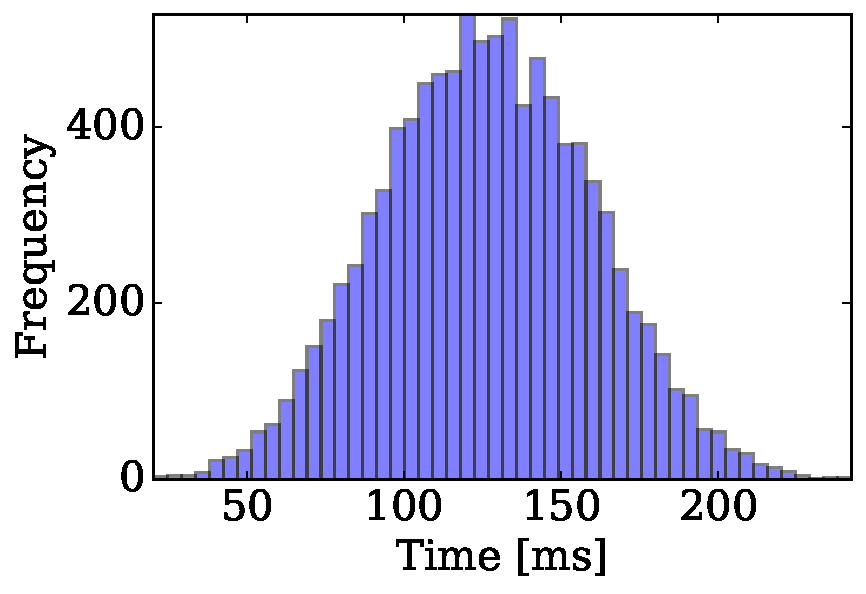
\includegraphics[clip, trim=0.2cm 0.3cm 0.2cm 0.2cm,scale=0.26]{TexImg/SF_query_dij_B25.pdf}
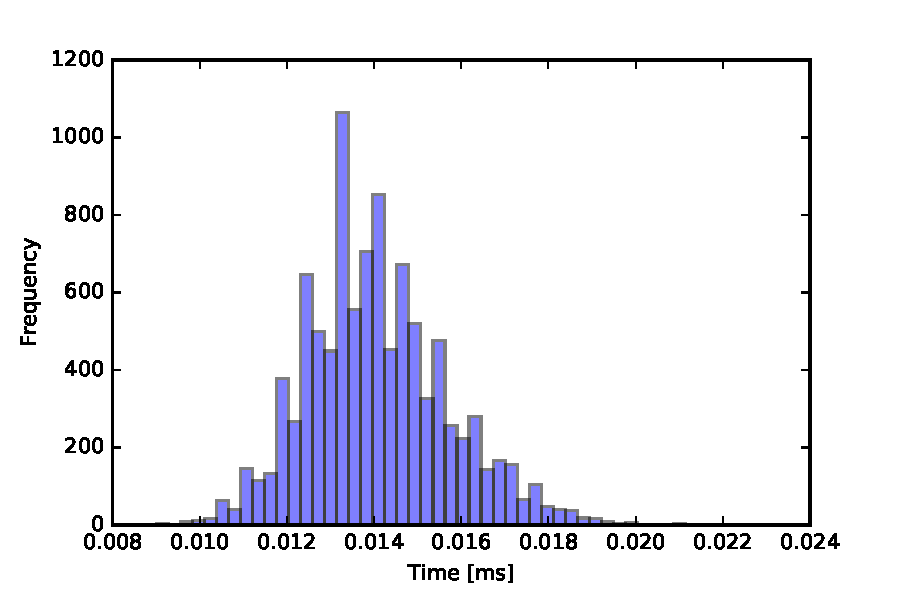
\includegraphics[clip, trim=1.3cm 0.3cm 0.2cm 0.2cm,scale=0.26]{TexImg/SF_query_hl_B25.pdf}
\end{center}
\caption{Histogram frontier queries in San Francisco augmented with $B=25$. Dijkstra (left) and HL (right).}
\label{fig:SF_query}
\end{figure}



\subsubsection{Hub sizes and node significance}

We focus the analysis on two meaningful quantities.
The first is hub size, which is well captured by  $\card{\Lb(\pp{t,0})}$ for $t\in V$.
Indeed, for frontier queries the reverse hub is bounding the space requirements; for specific queries the same is true up to a constant factor.
For the second quantity, we define the significance of $s\in V$ as the number of hubs containing $s$, i.e., $\sum_t\sum_b\In{\pp{s,b}\in \Lb(\pp{t,0})}$.
Intuitively, a node is highly significant if belongs to many efficient paths.
Figure~\ref{fig:SF_bwd_size} shows a histogram of these metrics. 

Figures \ref{fig:SF_hub_size_map} and \ref{fig:sig_colapse} show the spatial relationships between the hub size and significance in the San Francisco network. 
We observe that highly significant nodes tend to have small hub size.
The intuition is simple, if most hubs contain $s$, then is easier for $s$ to satisfy the cover property with a small hub.
Note also that the hub size resembles an harmonic function; nodes are mostly similar to their neighboors.

\begin{figure} 
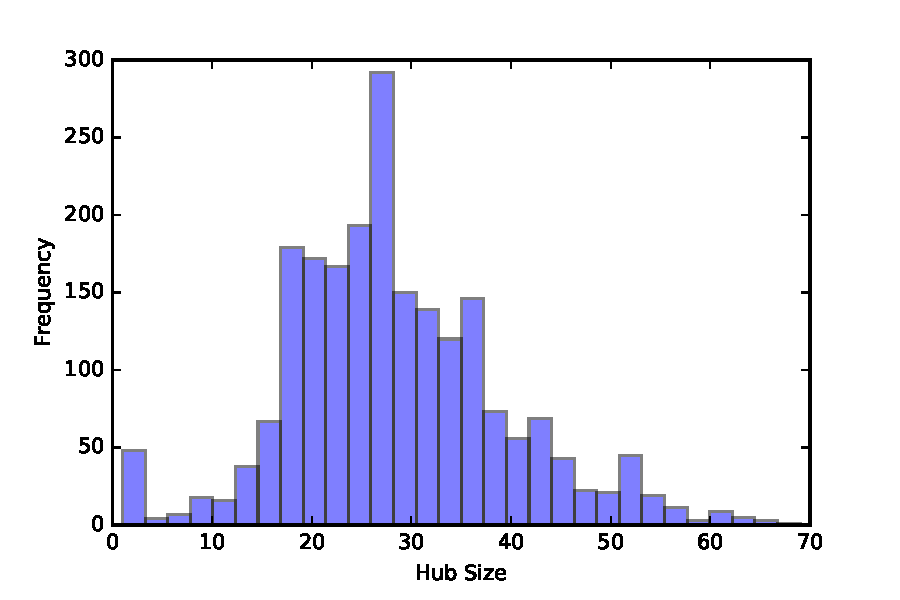
\includegraphics[clip, trim = 0.1cm 0.3cm 0cm 0cm,scale=0.27]{TexImg/SF_bwd_hub_size.pdf}
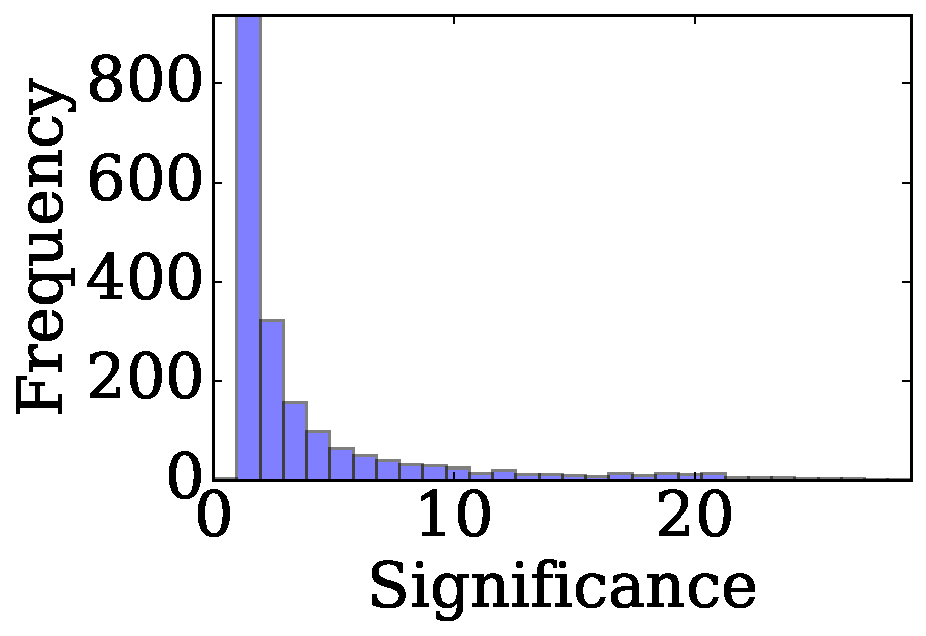
\includegraphics[clip, trim = 1.3cm 0.3cm 0cm 0cm,scale=0.27]{TexImg/significance.pdf}
\caption{Size of reverse hubs (left) and significance (right) for frontier queries in San Francisco augmented with $B=25$.}
\label{fig:SF_bwd_size}
\end{figure}
	
\begin{figure}
\begin{center}
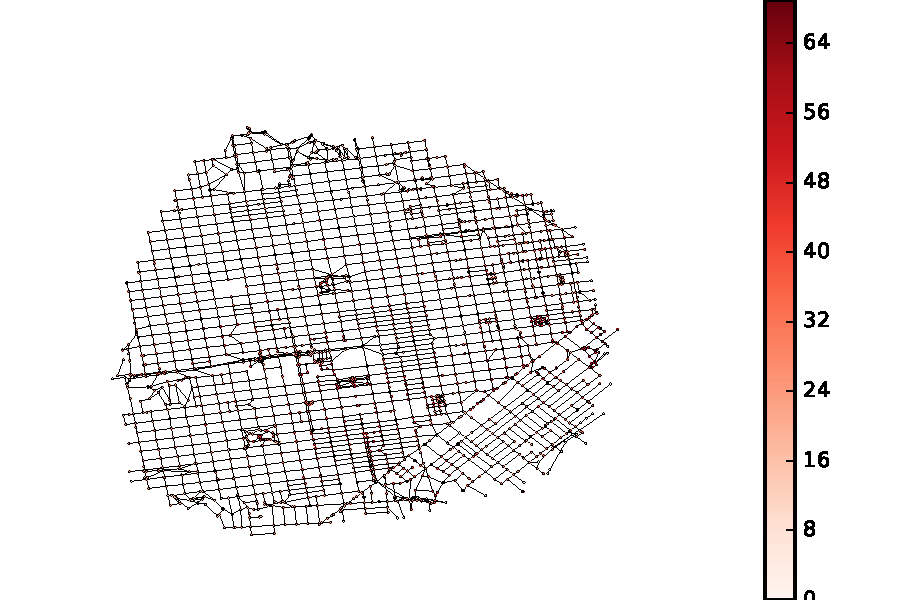
\includegraphics[clip, trim=4.5cm 4.8cm 4.7cm 3cm,scale=0.8]{TexImg/SF_hub_sizes.pdf}
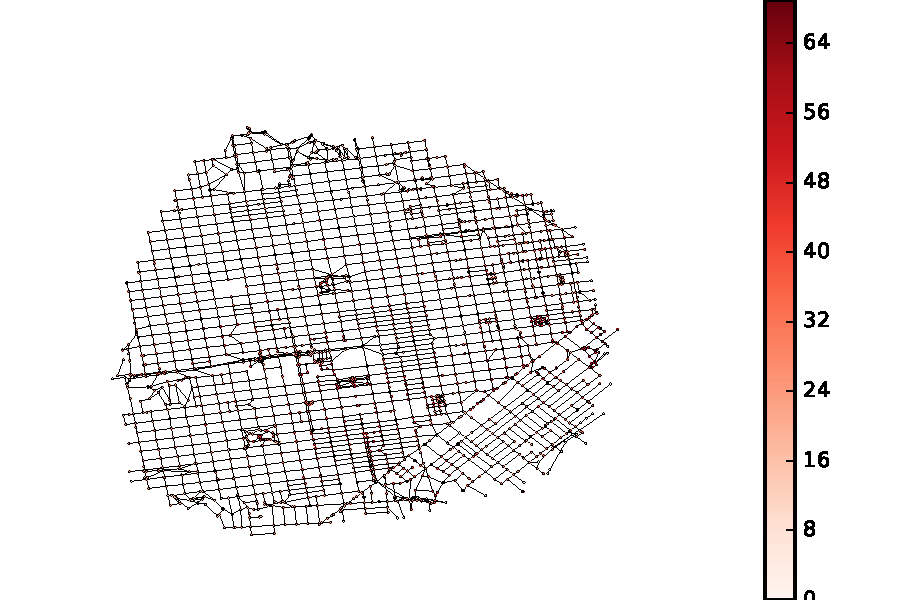
\includegraphics[clip, trim=15.8cm 0cm 0.4cm 1cm,scale=0.3]{TexImg/SF_hub_sizes.pdf}
\end{center}
\caption{Heat map of hub size for frontier queries in San Francisco augmented with $B=25$.}\label{fig:SF_hub_size_map}
\end{figure}

\begin{figure} 
\begin{center}
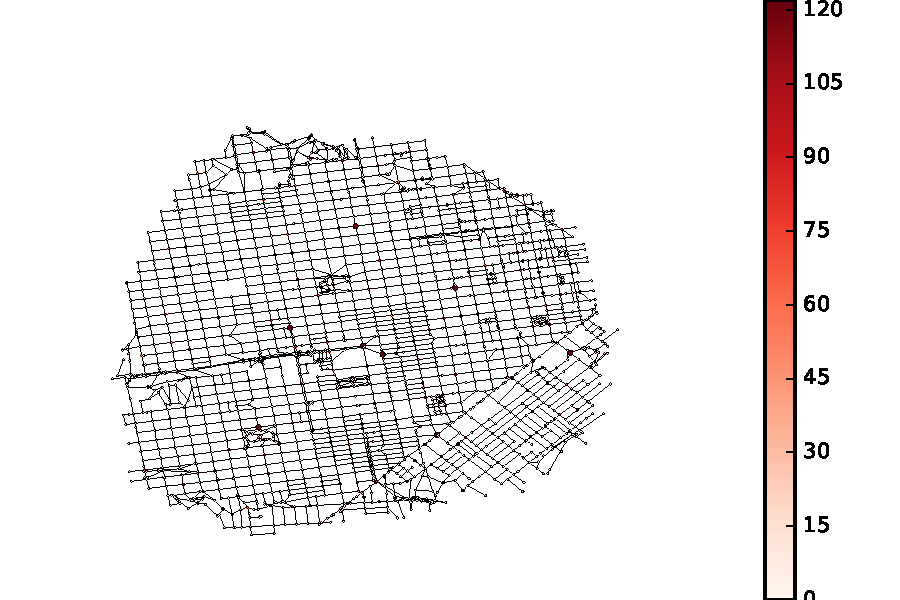
\includegraphics[clip, trim=3.7cm 2.9cm 4.2cm 3cm,scale=0.8]{TexImg/sig_colapse.pdf}
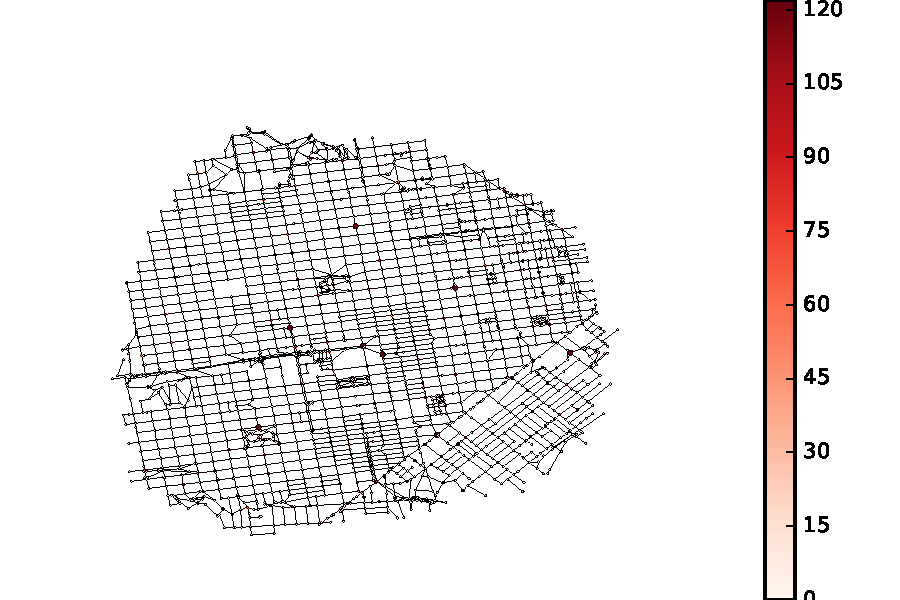
\includegraphics[clip, trim=15cm 1.5cm 0.1cm 0.8cm,scale=0.45]{TexImg/sig_colapse.pdf}
\caption{Heat map of significance for frontier queries in San Francisco augmented with $B=25$.
The most significant nodes have been drawn bigger.
The top 3 most significant correspond to Geary Blvd \& Gough St, Franklin St \& O'Farrel St and Market St \& Polk St.}
\label{fig:sig_colapse}
\end{center}
\end{figure}

\begin{figure}
\begin{center}
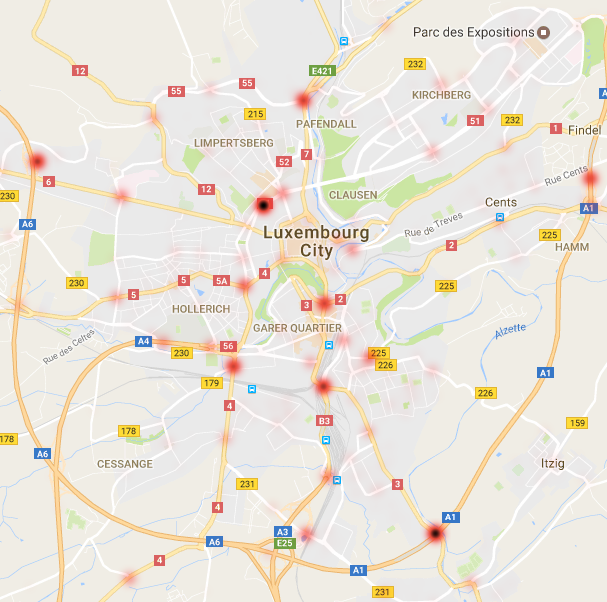
\includegraphics[scale=0.37]{TexImg/map_LU_sig.png}
\end{center}
\caption{Heat map of significance for frontier queries in Luxembourg City augmented with $B=25$.
Notice how the highly significant nodes are in main road crossings.}
\label{fig:map_LU} 
\end{figure}